\chapter{Left 4 Dead 2}

\section{Map Difficulty}
\begin{enumerate}
\item Bridge
\item Mall Atrium
\item Generator Room
\item Gator Village
\item Bus Depot
\item Stadium Gate
\item Sugar Mill
\item Underground
\item Concert
\item Riverbank
\item Motel
\item Plantation
\item Traincar
\item Port (S)
\item Port (P)
\item Rooftop (No Run)
\item Burger Tank
\end{enumerate}

\section{Weapons}
Contrary to the Left 4 Dead, Left 4 Dead 2 features a variety of range weapons that can be effectively used in survival mode. Also, the shotguns are a little underpowered. Because of their extremely short range, they are ill-suited for a lot of the long-range maps that are in Left 4 Dead 2. However, they still work decently.

\subsection{AK-47 Tactics}
The AK-47 is and extremely powerful gun but has accuracy problems.

\paragraph{Spray against tanks, burst against specials}
Tanks are large targets so rapid fire but low accuracy is fine to kill them. Against specials, burst fire towards the head is sufficient to kill them. Most common infected will die in one shot to AK-47 so a combination of burst and spray can be used depending on the situation.

\paragraph{Laser sights}
The AK is extremely powerful and accurate with laser sights. This makes is by far the best weapon to use. On the few survival maps that have AK-47 and laser sights, it should be used.

\subsection{Sniper Tactics}
The military sniper rifle is one of the most powerful weapons in Left 4 Dead 2 with the right usage. However, it is easily to use it improperly.

\paragraph{Scope to improve accuracy}
While running, the sniper is very inaccurate. However as soon as it is scoped, the player will slow down and the accuracy will quickly increase. A good way to quickly snipe zombies on the run is to scope in, shoot, and then scope out.

\paragraph{Spam against tanks}
Tanks are a huge target and the damage dealt to them does not depend on the area that you hit. Therefore, the sniper rifle should be fired as fast as possible (spammed) on the tanks in order to kill them. This requires a lot of clicking due to the nature of the sniper and it is tiresome, but any good sniper should get used to this.

\section{General Strategy}

\subsection{Ammo Runs}
In Left 4 Dead, there are breaks inbetween the waves of tanks. This is the opportunity when the survivors are able to make a run to replentish their ammo at the ammo pile. The times are:
\begin{itemize}
\item 1:30
\item 2:30 (optional)
\item 4:00
\item 6:00
\item 9:00
\item 12:00
\end{itemize}

These times are dependent upon what times the tanks spawn and die. If tanks spawn far away, they might interfere with the ammo runs. Likewise if the tanks are not killed fast enough.

After 12:00, the ammo runs are not set in stone, and tanks will come continuously. If the team is very efficient at killing the tanks, ammo runs will be possible inbetween tank spawns, and opportunities may open up at times such as $\sim$15:00 and $\sim$17:30.

\subsection{When to heal}
The correct time to heal is a subjective measure but it can greatly affect the outcome of the game.

\subsubsection{Pills, Adrenaline, and Medkits}
Pills give temporary health but are applied instantaneously whereas medkits give permanent health and take time. Medkits should be used when the health is low and there is sufficient time to heal. Pills should be used in times of emergency when you need an extra boost to prevent from getting incapacitated.

Adrenaline gives instant boost to the speed of all actions of the survivors. It allows you to outrun special infected and pick up survivors faster. However, it does not give a great bonus to your health. The adrenaline should be saved for crucial times such as when multiple survivors are incapacitated or a quick escape is necessary. It should not be used for normal healing purposes.

\section{Rules}
As explained in Section \ref{sec:rules1}, the rules are established for comparison and for friendly competition.

It should also be noted that the Left 4 Dead and Left 4 Dead 2 communities use different rules.

\begin{enumerate}
\item The use of mat-hacks, aimbots or any other tools that would result in a VAC ban from this game will obviously disqualify your time.
\item  Preventing AI (artificial intelligence) pathfinding, by either glitching out of the level, or using props or ammo packs to block the path will disqualify a time. AI do occasionally get stuck on their own free of player interference, as long as you can reasonably and relatively safely free/kill them you should try.
\item  The kill count for special infected (SI) must not deviate too far below the average expected kill count for any particular level (some levels, e.g.\ stadium gate, will have lower counts than others).
\item  The tank kill count must be at least 2 tanks per min (averaged from 13 mins onward) unless a kiting strategy was used, in which case, demo must be provided for the purpose of verification.
\item Moving items is allowed, but only if the item can be moved, e.g, it isn't possible to move all explosives on the sacrifice port before the round begins. However gun spawns may not be moved. PS. If using stripper configs, or the survival helper plugin beware of item counts and items from outside the playable area.
\item Scripts that assist gameplay or remove the need for a required skill (e.g.\ pistol scripts) are forbidden.
\item At the very least, for verification purposes, a screenshot should be provided, and if there is any dispute over the validity of the time, a demo from at least 1 player that partook in the run will be required for a time to be allowed to stand.
\item Players may customise their game too their liking so long as these changes do not detract the need for a certain skill, or give significant advantage otherwise not available without modification from a third party. This encompasses settings available through the games menus and console (commands which aren't cheat protected), which include, lerp, static/dynamic crosshairs, lowering graphical settings, changing the amount of audio channels. 
\end{enumerate}

Other, third party modifications that are allowed, are, custom huds, custom sound packs (as long as they don't just reduce the sound of guns and common infected to make si easier to hear), custom skins (weapons and survivors only), custom skyboxes.

It is well known that the in-game voice communication program is very low quality and suffers from lag. Third party communication programs, such as ventrilo \cite{web:ventrilo}, mumble \cite{web:mumble}, teamspeak \cite{web:teamspeak}, skype \cite{web:skype}, are allowed, as these do not offer any significant advantage over the in game chat.

\section{Dead Center}

\subsection{Mall Atrium}
Mall Atrium is a unique map because of its design. It includes three floors that the players can move around in and therefore gives players and most mobility and flexibility in terms of effective strategies. There are two types of strategies in this map: running and holding. The running strategy involves running from the tanks in a circuit and the hold strategies are like the other traditional strategies where the players try to kill all of the tanks. The easiest strategy to begin with is the running strategy.

\subsubsection{Bridge Hold (with stairs)}
This strategy involves holding the bridge but having one person on the stairway. The change in positioning radically changes the AI pathfinding and causes tanks to run up the stairs instead of climbing the columns as they usually do. This video shows roughly the strategy used however, it was more of an improvised/testing run so infact the strategy is more organized at this point: \url{http://youtu.be/mSrCbEguBIM}.

\paragraph{Positions}
See \figurename\ \ref{fig:bridge_hold_positions}
\begin{itemize}
\item 1 Player cover the top of the stairs (A)
\item 1 Player general/sniping (B)
\item 1 Player cover the bridge (C)
\item 1 Player on the stairs (D)
\end{itemize}
\begin{figure}[htb!]
\centering
\subfigure[Position for the stairs player. The player is optionally supplied with gascans and molotovs.]{
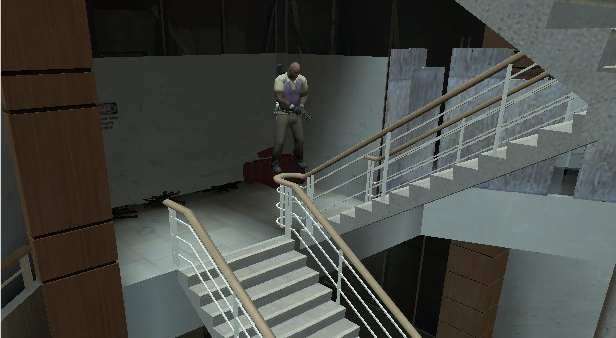
\includegraphics[width=0.45\columnwidth]{mall/mall_stairs}
\label{fig:mall_stairs}
}
\subfigure[Bridge hold positions. Most of the supplies are located in the corner by Player B.]{
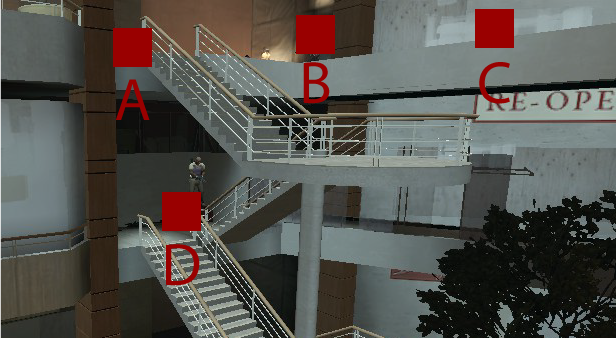
\includegraphics[width=0.45\columnwidth]{mall/mall_bridge_positions}
\label{fig:mall_bridge_positions}
}
\caption{Positions for bridge hold}
\label{fig:bridge_hold_positions}
\end{figure}

\paragraph{Notes}
\begin{itemize}
\item This positioning greatly frees up the space and freedom of movement on the top floor. However, the three top floor players must deal with the tanks without help from the fourth.
\item The player on the stairs has the most difficult position. He must fend off a lot of common zombies and avoiding getting hurt by specials and tanks going up the stairs
\item The player on the stairs must be carefully protected. The player guarding top should prevent zombies dropping at the top of the stairs onto him. Also do not bait tanks onto the stairs as this can be disasterous!
\item Depending on your positioning on the stairs, tanks will attack different. Move closer to the bottom and tanks will chase you up the stairs. Move close to the top and tanks will chase you up columns. Therefore, the stairs player has some control over the ebb and flow of tanks.
\item Gascans should be saved for the stairs player. The stairs player can kill a lot of zombies by flaming the stairs and baiting them to run through the fire.
\item Jockeys are difficult to deal with on the stairs and can cause you to take fall damage. The top floor players should lookout for the specials.
\item Players on the bridge need to watch for chargers that charge across the bridge.
\end{itemize}

\subsubsection{Saferoom Hold}
This is more of a hybrid strategy because it involves both running and killing the tanks. Many of the players refer to the third floor enclosed area as the saferoom. Some of us malls rats have been working on and tweaking a strategy, which involves holding your teams position inside the saferoom, killing tanks, and going for ammo when neccessary.

This strategy (or variation) is a combined effort of Mallrats and 24 carat survival
(\url{http://steamcommunity.com/groups/24CtS}).

\paragraph{Setup}

\subparagraph{Supplies}

Bring all supplies including guns to the saferoom. (not absolutely necessary, but makes it easier). Separate to your liking all the supplies such that they are easily accessible while playing under pressure.

\subparagraph{Gascans}

Place gascans between the crevasse. (Note: gascans are not necessary or this strategy to work; however, the more the supplies the easier it is).

\paragraph{Positions}
\begin{itemize}
\item 2 Snipers in front of the entry way, a little behind the wood walls such that tank rocks, and chargers will not stumble you.
\item 1 Shotgun that focuses 90\% of his/her attention on the back wall.

\item 1 Swivel position that switches between shotgun and sniper depending on where the tank comes from.
\end{itemize}

\paragraph{Description}

\begin{itemize}
\item Front Entry way (front)
\item Back wall (back)
\item Drop hole (hole)
\end{itemize}

2 Snipers ( or 3 if the swivel is required to help the front), take out special infected and common infected in the hallway. The back shogun must make sure that no common or SI (special infected) get through to bother the 2 or 3 front snipers, especially chargers and spitters. If these SI get in the way it can be game over when the tank attacks.

\subparagraph{Front Tanks}
If the tank comes from the front, 2 Front snipers and 1 Swivel focus fire it. A tank takes approximately 45 sniper rounds to kill, which means 15 rounds per sniper (or 1/2 a clip). If the tank is still alive when entering the saferoom and if the back is clear, the back shotgun can blast a couple shells in to finish the tank off.

\subparagraph{Back Tanks}
If the tank comes from the back, the back shotgun IMMEDIATELY has to call the tank in order to alert the swivel if he/she is facing the front. You will know 80\% of the time the tank is coming from the back if the ground starts rumbling. While the tank is climbing up the back shotgun and swivel blast the tank with 10 shells each through the wall. The swivel then moves quickly out of the way such that the tank will lock onto the back shogun. The back shogun proceeds to move backwards towards the hole but onto the ledge, without dropping down. Once the shogun has reached the corner, the tank cannot attack him/her and must then move around the hole (refer to hole dance). While this is happening 1 sniper (left sniper) is always facing the front to deal with SI or common.

\subparagraph{Hole dance}
This requires the left front sniper to lead the tank towards the hole. towards the back. You can prevent yourself from dropping down the hole by hugging the left wall and you backtrack. Once the tank reaches the front side of the hole and the player is on the other end the tank will attempt to go around and hit you on the other side. At that point you will want to move back towards the front on the ledge and repeat until the tank is dead.

\subparagraph{Ammo}
Ammo runs are possible at the third floor bridge ammo before 12 mins.
After 12 mins, call out when ammo is running low and on the next tank perform a conventional circuit.

\paragraph{Acknowledgements}
Perhaps many people have come up with variations on this strategy; however, I would like to give credit to those who helped develop this particular variation. Unfortunately I am uncertain of absolutely everyone involved, but anyone knows anything please let me know and I will add to the list.

\begin{itemize}
\item Piling guns in saferoom: murphy
\item 1 swivel position: reminiscence
\item The hole dance: guyguy
\item Tweaks/Testing: phoenix\_advance, guyguy, kev, lone wolf macgruber
\item Stress Testing: arkron, clutch, benanigans, jester, lemonman, flux, trash4cash, logankenesis
\item Circuit: Kris and the members of randomgroup21 (\url{http://steamcommunity.com/groups/randomgroup21})
\end{itemize}

Video Example: \url{http://www.youtube.com/watch?v=2fWy_tB2qug}

\section{Dark Carnival}

\subsection{Motel}
\paragraph{Positions} See \figurename\ \ref{fig:motel_positions}
\begin{itemize}
\item One player on the right (A)
\item Two players in the middle (B \& C)
\item One player on the left by the gascans (D)
\end{itemize}
\begin{figure}[htb!]
\centering
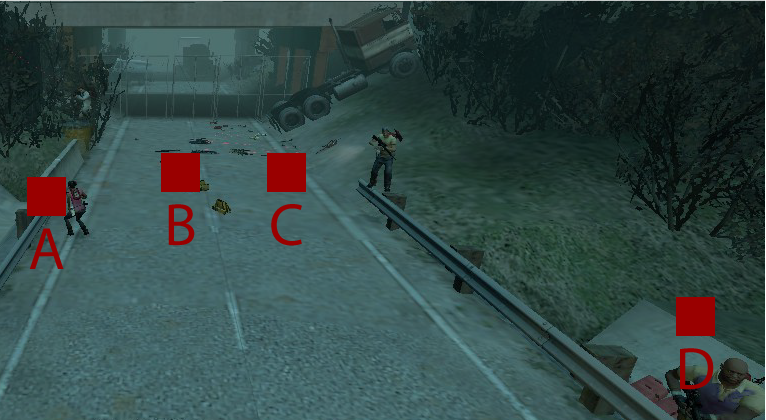
\includegraphics[width=0.7\columnwidth]{motel/motel_positions}
\caption{Motel positions}
\label{fig:motel_positions}
\end{figure}

\subsection{Stadium Gate}
\paragraph{Positions}
When holding the roof top of the barn near the AK47 face the other rooftops as front so we have:
\begin{itemize}
\item 1 Player at the right of the rooftop.
\item 1 Player at the left of the rooftop.
\item 2 Players in between on the rooftop.
\end{itemize}
Soon tanks overrun us resulting in a fall back to the AK47 spawn so we have:
\begin{itemize}
\item All 4 Players near close enough to the gun spawn to avoid reloading.
\end{itemize}

\paragraph{Tank Strategy}
\begin{itemize}
\item Gun down the common and tanks almost the same time.
\item Pick up a new AK47 when near the gun spawn.
\item Avoid rocks by shooting them or dodging them.
\item You can get around the same amount of si kills without holding the roof, just by killing infected during breaks. When you hold the roof they tend to get stuck elsewhere. Also a well placed molotov can kill the si that are stuck, but you'll probably need to practice the throw a bit to get use to the angle.
\end{itemize}
We have a lot of room for improvement and ideas on the way to get more SI kills safely. Next time we need to deal with rocks better and conserve medkits longer. Until next time, I suppose we can shoot for an hour or while we are at it the world record.

\subsection{Concert}
This map may have had the most changes in strategy not only due to the dispute over ladder-blocking, but the map changing all together. The map was updated around summer 2011. Since the update concert provided a better versus map, survival has had to adapt to new spawn points and old strategies crumbling. Although common infected are easy to kill and you'd rather focus on something like a special infected or tank(s), they serve an important role in the game. The combination of an endless horde, special infected, and tanks balance the games difficulty so removing one of these three would make a simple game. When all four play on the sniper tower it’s impossible for any common to play their role by blocking their climb. Not to mention the blocking of anything else climbing up. The description below is how we played concert to achieve the world record without blocking anything.

One player was on the sniper spawn scaffolding and did not block any ladders. The three other players played near the 2 medkits at the top of the bleachers. We played this way for the majority of the round but the first 9 mins we defended the stage in hopes of a better special infected count. Common infected may be funneled in by the guard rails near those 2 medkits so that one player is free of horde to focus on the tanks/SI while the other 2 focus on not letting common in. 

\paragraph{Positions}
See \figurename\ \ref{fig:concert_positions}. (Front is facing the stage from the top of the bleachers)
\begin{itemize}
\item 1 Player on the scaffolding spamming the sniper, shooting in all directions (A).
\item 1 Player is on the right funnel guard rail focusing the right and protecting the scaffolding player (B).
\item 1 Player is on the 2 medkits shooting in all directions (C).
\item 1 Player is on the left funnel guard rail focusing the left (D).
\end{itemize}

\begin{figure}[htb!]
\centering
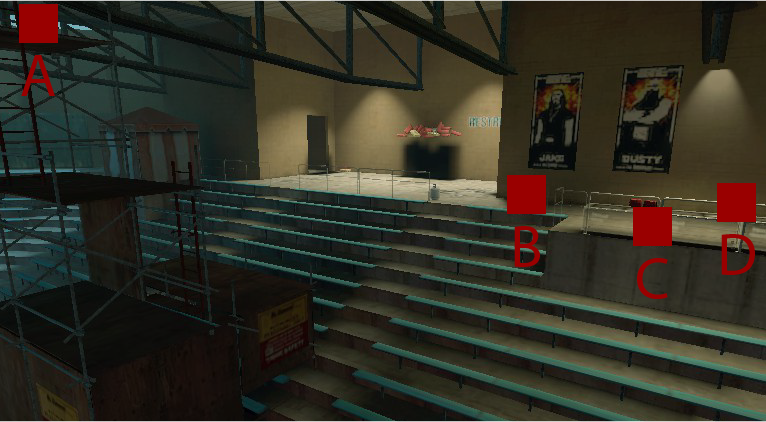
\includegraphics[width=0.70\columnwidth]{conc/concert_positions}
\caption{Positions for concert strategy}
\label{fig:concert_positions}
\end{figure}

\paragraph{Notes}
\begin{itemize}
\item The scaffolding player must be a stronger sniper with endurance to spam at the maximum speed the entire round.
\item The horde must be funneled in and prevented from slipping past for the ground players.
\item The ground players primarily used a military sniper to prevent running to the far ammo pile at the stage.
\item Keep the supplies near the vending machine with the gas on top of the vending machines (seen in \figurename\ \ref{fig:concert_positions}). The guns need to be where you funnel in the common.
\item When a player is down, a throwable must be used to pick that player up safely.
\item Gascans are a great way to kill a horde or light an unchipped tank. 
\item Since the middle ground player is mostly free of horde that player must be focusing the tanks and SI while helping with the horde when possible.
\item If the tank climbs up the scaffolding warn that player to escape before it’s too late.
\item Don’t wait until you’re out of ammo to get a new sniper, grab one when you’re on your last clip or after a double tank.
\item Calling the direction in which the tank is coming from will give you the best results, so construct your own front and back before the round starts so no one is confused.
\item If 2 or more players die it’s best to run around the perimeter of the map to stretch a couple mins.
\item Lots of spitters target the player on the scaffolding, so when there's spit just jump on the railing until the spit is gone.
\end{itemize}

\section{Swamp Fever}

\subsection{Gator Village}
\paragraph{Positions} See \figurename\ \ref{fig:gator_positions}.
\begin{itemize}
\item 1 player left bench (A)
\item 2 players middle (B \& C)
\item 1 player right bench (D)
\end{itemize}
\begin{figure}[htb!]
\centering
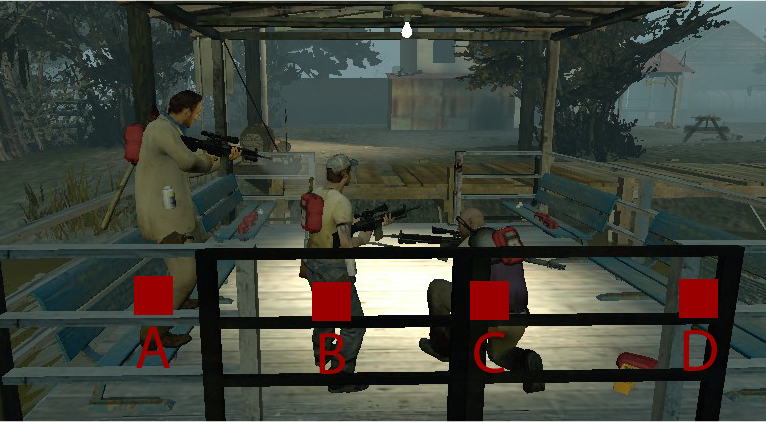
\includegraphics[width=0.7\columnwidth]{gator/gator_positions}
\caption{Positions on the barge for gator village}
\label{fig:gator_positions}
\end{figure}

All players use sniper rifles and stay on the barge once it arrives at about 2 minutes.

\paragraph{Notes}
\begin{itemize}
\item Judging by end-of-round statistics, the right player deals the most damage to the tank because he has the best view of the tank. Other players have their view obstructed in most cases.
\item In the case of two tanks, the right player can chip at the second tank while the main players deal with the first (closest) tank.
\item Since the leftmost player has easy access to the sniper rifle, it seems he's able to deal with most common infected.
\item Dodging rocks is important to conserving health as it is in most other maps. While it's difficult to avoid getting hit in some cases, players should try to position themselves so that the rocks miss their target or break against the poles of the barge.
\end{itemize}

If the players are strong enough snipers, the team won't need to use any other weapons other than sniper rifle. There is enough time to snipe the tanks before they reach the barge. Admittedly, this map is very tiresome and also it makes you improve at sniping in Left 4 Dead 2

\subsection{Plantation}
No information written yet.

\section{Hard Rain}

\subsection{Sugar Mill}
\paragraph{Positions}
\begin{itemize}
\item 1 player by the ammo pile spamming the SCAR-L and shotgun
\item 2 players behind the back of the truck using sniper rifles. Some people play it with 1 crouched in the front and 1 standing behind them, but friendly fire seemed to be a problem as the player in the front crouching moves a bit and gets in the back player's line of fire while moving. So the 2 truck players crouched side by side.
\item 1 player watching the back and helping with tanks in the front if the back is clear.
\end{itemize}

%By about 30 minutes we had used all of our gascans, so we started tossing mollies when needed. By 45 minutes we still had 6 kits, 2 defibs, 6 adrenaline, and 4 sets of pills left (not including what was on our backs). When the back was clear, the back player crouched on the left side of the truck and had a good view of the far front under the truck, so he was chipping tanks for us. Melee weapons > pistols for this map.

\paragraph{Notes}
\begin{itemize}
\item When we had doubles and the tanks were coming in close, we backed up to the dead end.
\item It is important for the front bait player to dodge rocks. It's particularly the rocks coming from the left-side tanks that we seemed to have some trouble with. 
\item The back player can have some pretty smooth moves. She can manipulate the tank to chase her in a circle on the corner of the concrete. She can make it climb up then come back down and climb up again a couple of times. It buys the survivors a little bit of time if they also have zombies to deal with in the front.
\item The front bait player usually gets spat on, so it's very important for them to back up in time to not take damage, and for the 2 truck snipers to warn him of the specials and rocks coming from the front.
\item Sometimes specials and even tanks will drop on you.
\item Health and throwables were moved and stored in the back dead-end corner, because the previous attempt before this we had a boomer in the back explode and all our supplies blew away.
\end{itemize}

\subsection{Burger Tank}
\paragraph{Positions}
See \ref{fig:bt_positions}.
\begin{itemize}
\item One player on the front left (A)
\item One player front middle (B)
\item One player front right (C)
\item One player on the chimney (D)
\end{itemize}
All players are using the sniper rifle and replentishing ammo at the sniper spawn. All of the players need to be proficient at the sniper rifle because it is a very difficult map. The left player is controlling most of the horde that climbs up on the left side and also watching for any special infected climbing the left side of the building. The other front players are dealing with the zombies they encounter and also shooting the tanks. The back player is watching over all of the other players, keeping the zombies from attacking them from behind. The back player also has to watch the back side for special infected that sometimes come from the back or from up the ladder.

\begin{figure}[htb!]
\centering
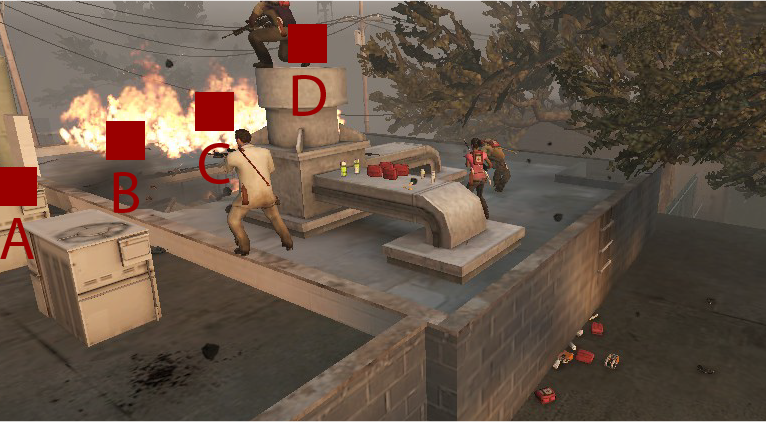
\includegraphics[width=0.70\columnwidth]{bt/bt_positions}
\caption{Positions for burger tank roof strategy}
\label{fig:bt_positions}
\end{figure}

\paragraph{Notes}
\begin{itemize}
\item There are a lot of health items, particularly medkits, on this map. There is no need to use the health sparingly.
\item Burger tank has a frantic pace after twelve minutes. It is very difficult to keep control of the roof.
\item There are two bile jars that should be saved for emergencies.
\item The gascans should be stored in a place where they will not be destroyed. Some good places are in the corner by the left player and on the side by the right player.
\end{itemize}

\section{The Parish}

\subsection{Bus Depot}
%We've had some recent success in Left 4 Dead 1 and 2 and some new records, which means there will be a few new announcements forthcoming. It's hard to say whether this is a world record or not since the Japanese versus players have gotten 70 minutes on this map with much lower SI counts. At the very least, this is the second longest time recorded on this map.

%We used the tower defense strategy that phoenix and friends developed. It's well-documented in this youtube video: http://youtu.be/H3H-OFGGV-E . It's a difficult strategy but our team has very strong sniper players.

\paragraph{Positions}
\begin{itemize}
\item 2 players at the tower
\item 1 player on the scaffolding near the front
\item 1 player on the fence
\end{itemize}
All players use sniper rifles. Items were moved for easy accessibility.

\paragraph{Notes}
\begin{itemize}
\item Good communication is essential for this strategy because during double tanks, we divide the focus of the players between the two tanks.
\item The two players at the tower can deal with back tanks with very little help.
\item The player at the fence has to deal with the front tanks and specials coming from the front. He can lead the tank in circles by making small movements along the fence.
\item The player at the scaffolding serves to backup the side that needs help.
\item We used a lot of the fire in the first 30 minutes.
\item All players use the sniper spawn to replentish their ammo.
\item It seems that the faster the tanks die, the easier this strategy has become. This requires a lot of shooting.
\item For the front player, he is playing on the fence to bait the tanks but retreating to the tarp to avoid rocks.
\item The back players are spamming the sniper rifle and they alone should be able to kill all back tanks and even double tanks at back.
\item According to statistics, the back players are doing the brunt of the damage to the tanks.
\item We improved on the amount of times falling off the fence and scaffolding. We used throwables whenever someone fell in order to recover.
\item The fence player moved to the tarp, where he was healed by the players on the tower. The fence player required the most medkits (that was me :P)
\item When it is clear, the fence player is clearing the front scaffolding of zombies and especially chargers climbing the scaffolding.
\item Special infected will sometimes move from the back through the alley to the front. In this case, the back players gave warning.
\item The roof tanks were getting killed by mostly the back players with help from the front scaffolding player.
\end{itemize}

The weakness of the strategy is that when players fall off the fence or scaffolding, it can be difficult to recover. We had little problems with this until the end, where we wiped out at 55 minutes despite having about 3 medkits and 1 defibrillator left. An hour is definitely possible with this strategy, which phoenix actually predicted, yet nobody believed him!

\subsection{Bridge}
This is the easiest map to play in all the maps of Left 4 Dead and Left 4 Dead 2. It is possible to last on this map indefinitely. The longest players have lasted here is five hours, with the rounds ending due to exhaustion.
\paragraph{Positions}
All players are lined up upstairs by the M16 spawn on the floor.

\section{The Passing}

\subsection{Riverbank}
In this map, extra medkits are dropped by special survivor zombies.

\subsection{Underground}
In this map, extra medkits are dropped by special survivor zombies. Note that this map has two names: Underground and Bedlam.

\subsection{Port}
No information written yet.

\section{The Sacrifice}

\subsection{Traincar}
\paragraph{Positions}
\begin{itemize}
\item 2 players on left boat, 2 players on right boat
\item Positions are not fixed after 12 minutes
\end{itemize}

\paragraph{Notes}
\begin{itemize}
\item We stay on top of the two boats in the middle. Some care must be taken to prevent damage when the boats break.
\item Retreat to the corner of the map once the tank/zombies make the boats too hectic. (This corner is the spot commonly used in L4D1 traincar)
\item We got a moderate supply of bile jars during this run. The bile drops are random; sometimes you can collect over 12 bile jars during the first 12 minutes.
\item Bile lasts about 20 seconds. It can alleviate you from the horde and special infected.
\item In this attempt we threw the bile jars on the ground near the ammo. The reasoning is to syphon the zombies to one spot, so more bile can be collected. Another possibility is to throw the bile on the tanks.
\item AK47 with laser sights is very powerful and accurate. It takes only 1 bullet to kill a zombie.
\item 1 designated player threw most of the bile on the ground to draw the horde of commons. It also allowed us to collect more bile.
\item If I remember, we had a moderate amount of bile before 12 minutes but gained a constant supply after 12 minutes.
\item Occaisionally, bile was thrown on tanks during dangerous times.
\item We retreated to the corner as the tank approached, but had problems with friendly fire during this time
\item Dodging rocks helped preserve health and allowed us to take minimal damage from tanks
\item We waited until about red health to heal. We used about 1 or 2 medkits by the time of 12 minutes.
\end{itemize}

\subsection{Port}
%This map uses a circuit strategy that we have recently been trying to improve on. Here are two old videos showing the strategy, although there have been some changes e.g. camping the pool room the first 12 minutes instead of the bar: http://www.youtube.com/watch?v=HTavXC9RGaY , http://www.youtube.com/watch?v=rOe9Fye7MqM

\paragraph{Positions}(Front is facing the lower level of the bar.)
\begin{itemize}
\item 1 Player front left
\item 1 Player front right
\item 1 Player front middle
\item 1 Player back
\end{itemize}

\paragraph{Notes}
\begin{itemize}
\item We hold for the first 12 minutes to collect bile jars. Running the circuits occurs after 12 minutes.
\item If the front players are positioned properly, the tank from the front will always climb to the second floor, making him an easy target.
\item The back player must be alert for specials dropping off the roof and climbing the nearby fence. It may be tempting to go outside the room, but I find that it is a risk to go outside where it is hard for your teammates to save you.
\item 3 players should shoot the tank and 1 player should cover the remaining side. Using fire to help cover is very useful.
\item The circuit starts from the pool room where we bile the tank and run usually out the back.
\item Once everyone has met up in the second building (warehouse), we wait for the tank and bile it again for the return trip to the pool room. There is a good chance that more bile can be found on the way through the circuit.
\item If you run out of bile jars, substitute with pipe bombs.
\item The back player may have to use 1 medkit within 12 minutes. The rest of the medkits must be used during the run.
\end{itemize}

\section{No Mercy}

\subsection{Generator Room}
Since the map is glitchy, many specials get stuck at an unreachable place during long games. The spitters getting stuck will greatly aid your team. However, we think the SI counts are reasonable enough.

\paragraph{Positions}
\begin{itemize}
\item 2 players at the front
\item 2 players at the back pressed up against the railing
\end{itemize}

No items moved. We used 4 medkits by 12 minutes.

\paragraph{Notes}
\begin{itemize}
\item The map will either spawn with laser sights or special ammo. The laser sights increase accuracy and make the AK47 very powerful, whereas the special ammo allow you to move the spare medkits to the top floor if desired. Using the laser sights seemed to help us save health even more than spare medkits would.
\item The back players are pressed up against the railing so that spit will bounce off of them. We did not need to worry about this after the spitters got stuck.
\item The tanks at the ground floor tend to throw rocks at the back players and the tanks at the top floor tend to throw rocks at the front players. The players need to be positioned to avoid taking damage from rocks.
\item In the case of double tanks, we approximately had the 2 front players focus on the closest tank while the back two players focused on the second tank.
\item Occasionally tanks will either spawn at the rear or jump out the window and run through the rear. These tanks are quite dangerous and should be dealt with quickly.
\item We went for ammo at frequently at convenient times instead of when our ammo was low.
\end{itemize}

\subsection{Rooftop}
No information written yet.
